\section{Appendix}
\subsection*{Functional Analysis}
A real vector space VV is a set with operations +:V×V→V+ : V \times V \to V and ⋅:R×V→V\cdot: \mathbb{R}\times V \to V such that:

\begin{itemize}
    \item u+v=v+uu + v = v + u (commutativity of vector addition)
    \item (u+v)+w=u+(v+w)(u + v) + w = u + (v + w) (associativity of vector addition)
    \item There exists an element 0∈V0 \in V such that v+0=vv + 0 = v for all v∈Vv \in V (existence of zero vector)
    \item For every v∈Vv \in V, there exists an element −v∈V-v \in V such that v+(−v)=0v + (-v) = 0 (existence of additive inverses)
    \item λ⋅(u+v)=λ⋅u+λ⋅v\lambda \cdot (u + v) = \lambda \cdot u + \lambda \cdot v (distributivity of scalar multiplication over vector addition)
    \item (λ+μ)⋅v=λ⋅v+μ⋅v(\lambda + \mu) \cdot v = \lambda \cdot v + \mu \cdot v (distributivity of scalar multiplication over real addition)
    \item (λμ)⋅v=λ⋅(μ⋅v)(\lambda \mu) \cdot v = \lambda \cdot (\mu \cdot v) (associativity of scalar multiplication)
    \item $1 \cdot v = v$ (scalar multiplication identity)
\end{itemize}


Examples of real vector spaces are: $\mathbb{R}^n$, $P_K(I)$: set of polynomials of order $\leq K$ on the interval $I$, $C^k(I)$: set of functions with $k$ continuous derivatives on the interval $I$.\\

A basis for the vector space $V$ is the minimal set of vectors (basis function) that span $V$. The basis functions must be \textbf{linearly independent} and the number of basis functions is the \textbf{dimension} of the vector space. Any vector $v \in V$ can be written as a linear combination of the basis functions:
\[
    v = c_1 \phi_1 + c_2 \phi_2 + \dots + c_n \phi_n    
\]

\textbf{Example}: the dimension of $P_K)I=$ is $K+1$ and the basis functions are $\{1,x,x^2,\dots,x^K\}$.\\

Let $V$ be a vector space over $\mathbb{R}$. An inner product $(,)$ is a function $V \times V \to \mathbb{R}$ with the following properties:
\begin{enumerate}
    \item $\forall u \in V, (u,u) \geq 0 $ and $(u,u) = 0 \iff u = 0$
    \item $\forall u,v \in V, (u,v) = (v,u)$
    \item $\forall u,v,w \in V$ and $\forall \alpha,\beta \in \mathbb{R}, (\alpha u + \beta v, w) = \alpha(u,w) + \beta(v,w)$
\end{enumerate}
$V$ together with $(,)$ is called an \textbf{inner product space}.\\

\textbf{Example}: Given two vectors in $\mathbb{R}^2: v = v_1e_1 + v_2e_2$ and $w = w_1e_1 + w_2e_2$, the Euclidean inner product in $\mathbb{R}^2$ is:
\[
    (v,w) = v_1w_1 + v_2w_2     
\]
The extension to $\mathbb{R}^n$ is obvious.\\

\textbf{Example}: An inner product in the vector space of continuous functions in [0,1] ($C([0,1])$) is:
\[
    (f,g) = \int_0^1 f(x)g(x)dx    
\]
where $f,g \in C([0,1])$.\\

\textbf{Example}: An inner product in the vector space of functions with one continuous derivative in [0,1] ($C^1([0,1])$) is:
\[
    (f,g) = \int_0^1 f(x)g(x) + f'(x)g'(x)dx    
\]
where $f,g \in C^1([0,1])$.\\

\textbf{Remark}: an inner product induces a norm $\|f\| = \sqrt{(f,f)}$.\\

A norm on a vector space $V$ is a mapping $\|\cdot\|: V \to \mathbb{R}$ that satisfies:
\begin{enumerate}
    \item $\|u\| \geq 0$ and $\|u\| = 0 \iff u = 0$
    \item $\|\alpha u\| = |\alpha|\|u\|$
    \item $\|u+v\| \leq \|u\| + \|v\|$
\end{enumerate}
This is valid $\forall u,v \in V $ and $\forall \alpha \in \mathbb{R}$.\\
A normed vector space is a vector space equipped with a norm. 
\begin{itemize}
    \item Norms in $\mathbb{R}^n$:
    \[
        \|v\|_p = \left(\sum_{i=1}^{n} |v_i|^p\right)^{1/p}   \hspace{1cm} \|v\|_1 = \sum_{i=1}^{n} |v_i| \hspace{1cm} \|v\|_\infty = \max_{i=1,\dots,n} |v_i|
    \]
    \item Norms in $C^0(I)$ and $P_K(I)$:
    \[
        \|v\|_{L^p(I)} = \left(\int_I |v|^p dx\right)^{1/p}   \hspace{1cm} \|v\|_{L^{\infty}(I)} = \sup_{x \in I} |v(x)| 
    \]
\end{itemize}

A \textbf{bilinear form} on a vector space $V$ is mapping a $a(\cdot,\cdot) = V \times V \to \mathbb{R}$ such that:
\begin{itemize}
    \item $a(u+v,w) = a(u,w) + a(v,w)$
    \item $a(u,v+w) = a(u,v) + a(u,w)$
    \item $a(\lambda u, v) = \lambda a(u,v)$
    \item $a(u,\lambda v) = \lambda a(u,v)$
\end{itemize}
This is valid $\forall u,v,w \in V$ and $\forall \lambda \in \mathbb{R}$. The bilinear form is symmetric if $a(u,v) = a(v,u)$ $\forall u,v \in V$ and continuous, or bounded, if there is a constant $C$ such that $|a(u,v)| \leq C\|u\|\|v\|$ $\forall u,v \in V$.\\

A symmetric bilinear form $a(\cdot,\cdot)$ is called an inner product if $a(u,u) \geq 0$ with equality if and only if $u=0$ $\forall u \in V$. Inner products are often also denoted $(\cdot,\cdot)$. An inner product defines a so-called induced norm by:
\[
    \|u\|^2 = (u,u)    
\]
on the vector space $V$. In particular, $a(\cdot,\cdot)$ defines the induced energy norm $\||u\||^2 = a(u,u)$. A vector space equipped with an inner product is called an inner product space. In such spaces the Cauchy-Schwarz inequality:
\[
    |(u,v)| \leq \|u\|\|v\|    
\]
holds for all $u,v \in V$.\\

A \textbf{Cauchy sequence} in a normed vector space $V$ is a sequence $\{v_i\}^{\infty}_{i=1}$ of elements $v_i \in V$ such that
 \[
    \forall \epsilon > 0 \hspace{0.2cm} \exists N \in \mathbb{N} \hspace{0.2cm}\text{such that}\hspace{0.2cm} \|v_i - v_j\| < \epsilon \hspace{0.2cm}\forall i,j \geq N
\] 
A normed vector space is called complete if every Cauchy sequence in $V$ converges to an element in $V$.\\

\textbf{Remark}: a convergent sequence is a Cauchy sequence. The converse is not true. Indeed, there are Cauchy sequences that do not converge in their space. For example, the sequence of rational numbers $(u_n)_{n \in \mathbb{N}} \in \mathbb{Q}$ given by:
\[
    u_n = \dfrac{1}{0!} + \dfrac{1}{1!} + \dots + \dfrac{1}{n!}    
\]
is Cauchy in $\mathbb{Q}$ but converges to the constant $e$, which belongs to $\mathbb{R}$ but not to $\mathbb{Q}$.\\

\textbf{Definition:} a vector space is said to be complete if every Cauchy sequence is also convergent.\\

\textbf{Definition:} a Banach space is a complete normed vector space.\\

\textbf{Definition:} a Hilbert space is a complete inner product space.\\

\begin{center}
    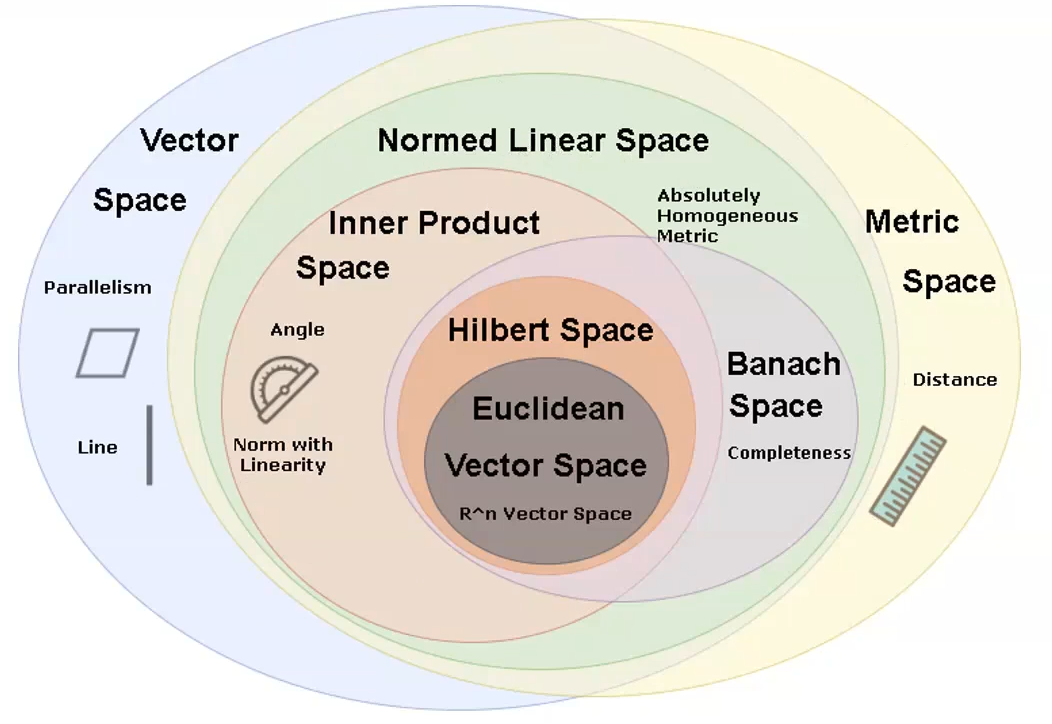
\includegraphics[scale = 0.2]{../images/SetsSpace.png}
\end{center}

\subsection*{Riemann integral}
For a function to be Riemann integrable, the infimum of the upper Riemann sum and the supremum of the lower Riemann sum should be the same.
\[
    m_k = \inf\{f(t):x_{k-1} \leq t\leq x_k\} \hspace{1cm} M_k = \sup\{f(t):x_{k-1} \leq t\leq x_k\}    
\]
\[
    L(f,P) = \sum_{k=1}^N m_k(x_k - x_{k-1}) \hspace{1cm} U(f,P) = \sum_{k=1}^N M_k(x_k - x_{k-1})    
\]
Is Riemann integral ok? Consider:
\[
    \mathbbm{1}_{\mathbb{Q}} = \begin{cases}
        1 & x \in \mathbb{Q}\\
        0 & x \notin \mathbb{Q}
    \end{cases}    
\]
In this case: $L(f,P) = 0 \neq 1 = U(f,P)$. So the function is not Riemann integrable. 

\subsection*{Lebesque integral}
Is defined as follows: 
\[
    \int_{\mathbb{R}}\phi dm := \sum_{i=1}^{n} a_i m(S_i)    
\]
Here, instead of having a partition of the interval, we have a partition of the set. The function $\phi$ is the characteristic function of the set $S_i$ and $a_i$ is the value of the function in the set $S_i$. \textbf{We are still computing a "rectangular" area but this time the base is not fixed to a certain "dx" (or $\Delta x$) but it is the measure of the set $S_i$ which can be large. The total area is not computed by stacking side to side small and tall rectangulars but by stacking on over the other larger and shorter (of height $a$)rectangulars}.\\
\begin{multicols}{2}
    \begin{center}
        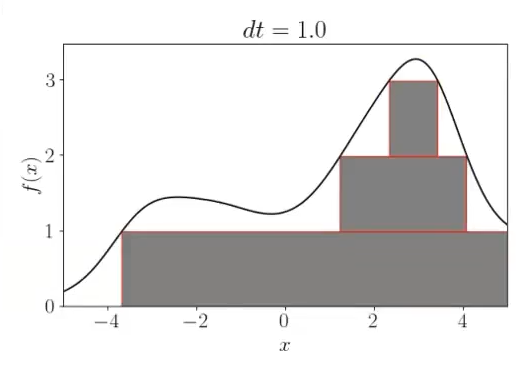
\includegraphics[scale = 0.4]{../images/LebesgueIntegral.png}
    \end{center}
    \begin{center}
        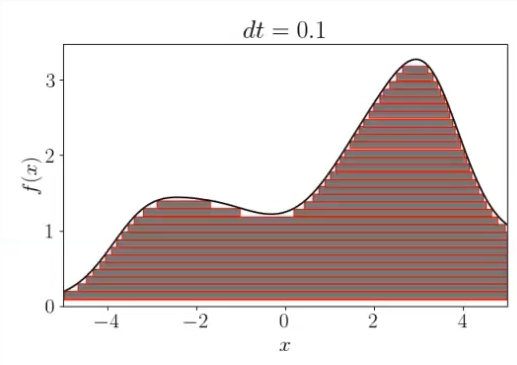
\includegraphics[scale = 0.4]{../images/LebesgueThinner.png}
    \end{center}
\end{multicols}
Of course, as it was done in Riemann integral, you will reach a better approximation of the area by considering thinner and thinner layers of rectangulars.
\textbf{We need to define the concept of "measure"!}\\

\textbf{Theorem:} every countable set has measure 0.\\

The integral with Lebesque is easy: $1\times S_1 + 0\times S_2$ where $S_1$ is the set of all irrational numbers in [0,1] and $S_2$ is the set of rational numbers. $S_2$ is countable so $\mu(S_2) = 0$ moreover since $S_1$ and $S_2$ are disjoint we have $\mu([0,1]) = 1 \implies \mu(S_1) = \mu([0,1] - \mu(S_2)) = 1 - 0 = 1$. So the integral is 1!

\textbf{Remark:} if a function is Riemann integrable then it is also Lebesque integrable and the two integrals coincide. The converse is not true.\\

With the Lebesque integral we can define the $L^p$ spaces:  
\[
    L^p(|\Omega) = \{v: \Omega \to \mathbb{R}: \|v\|_{L^p(\Omega)} < \infty\}    
\]
So the space $L^p$ is the set of functions which have norm which is bounded. The norm is defined as:
\[
    \|v\|_{L^p(\Omega)} = \left(\int_{\Omega} |v|^p dm\right)^{1/p}
\]
With $1 \leq p \leq \infty$. In particular, if $p = \infty$ we have:
\[
    \|v\|_{L^\infty(\Omega)} = \sup_{x \in \Omega} |v(x)|    
\]

\textbf{Remark:} the $L^p(\Omega)$ spaces are Banach spaces for $1 \leq p \leq \infty$.\\

\textbf{Remark:} The space $L^2(\Omega)$ is a Hilbert space, as its norm $\|v\|_{L^2(\Omega)}$ is induced by the inner product $(v,w)_{L^2(\Omega)} = \int_{\Omega} vw \, dx$. However, for $p \neq 2$, the space $L^p(\Omega)$ is only a Banach space, as its norm $\|v\|_{L^p(\Omega)}$ is not induced by an inner product.
\begin{center}
    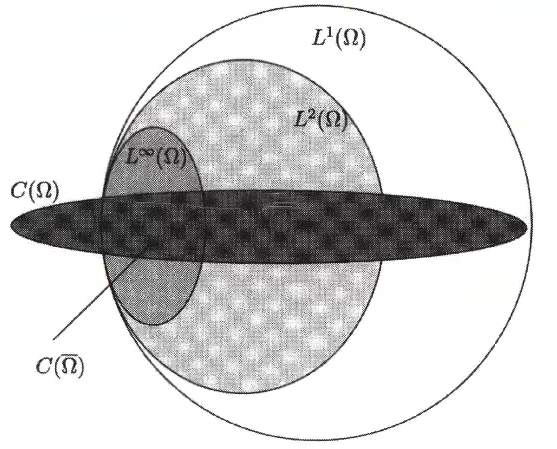
\includegraphics[scale = 0.35]{../images/LpSpaces.png}
\end{center}
In the picture there is also $C(\Omega)$ which corresponds to the set of continuous functions in $\Omega$. $\bar{\Omega}$ is the closure of $\Omega$.\\

Suppose have this differential problem:
\[
    \begin{cases}
        -u''(x) = f(x) & x \in (0,1)\\  
        u(0) = u(1) = 0
    \end{cases}    
\]
This, for example, is a model for an elastic string and $f$ is some sort of external force applied to it. We have 3 different external forces as shown in the figure here:
\begin{center}
    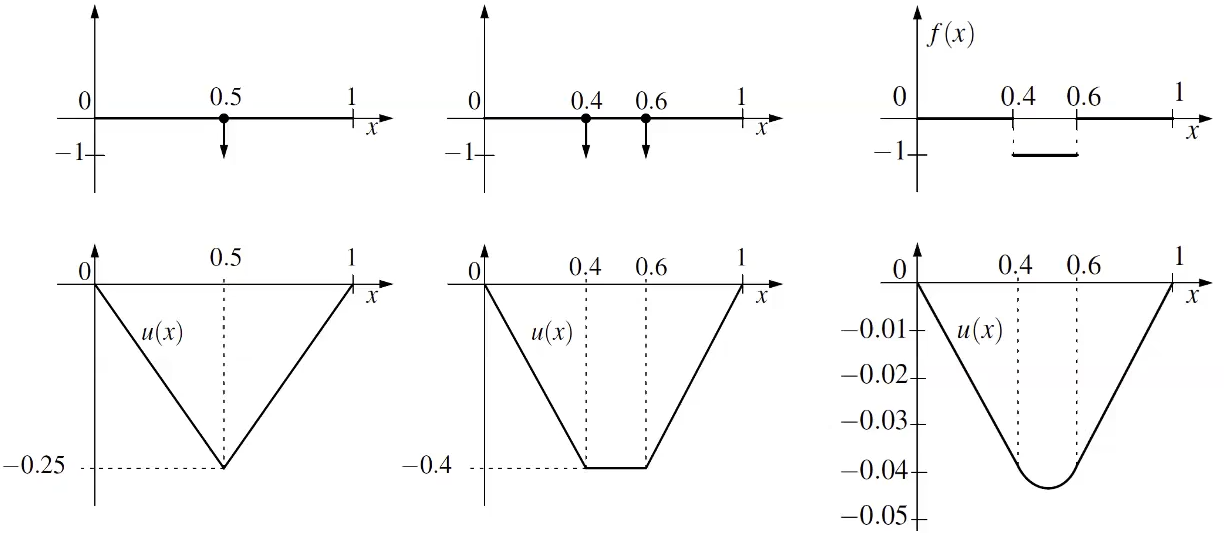
\includegraphics[scale = 0.35]{../images/ExternalForces.png}    
\end{center}
In the first case the force is all concentrated in the point 0.5, in the second case the force is distributed in the two points 0.4 and 0.6 while in the third case the force is distributed in the whole interval.In the bottom of the picture there are the solutions of the three problems. But, as you can see, the functions $u(x)$ are not differentiable.

There is a contraddiction: the physical problem admits a solution which is not coherent with the regularity required by the differential problem. We have to rethink the definition of derivative, we have to introduce the concept of \textbf{weak derivative}.\\

\subsection*{Weak derivatives}
Functions in Hilbert spaces are not regular enough for the standard definition of derivative to make sense. 
\begin{itemize}
    \item $C^k(\Omega)$: space of all $k < \infty$ times continuously differentiable functions in $\Omega$.
    \item $\mathcal{D}(\Omega) = \{\varphi \in C^\infty(\Omega) \text{with compact support in }\Omega\}$
    \item $\alpha = (\alpha_1, \dots, \alpha_d)$ is a multi-index, i.e. d-tuple of non negative integers
    \item $|\alpha| = \alpha_1 + \dots + \alpha_d = \sum_{i=1}^{d} \alpha_i$: order of the multi-index
    \item $D^\alpha \phi = \prod\limits_{i=1}^{d}\left(\dfrac{\partial}{\partial x_i}\right)^{\alpha_i} \varphi$, \hspace{0.1cm} $\varphi \in \mathcal{D}(\Omega)$
\end{itemize}
So, if we have to compute $\frac{\partial u}{\partial x_i}$ we can:
\[
    \int_{\Omega} \dfrac{\partial u}{\partial x_i} \varphi dx =  - \int_{\Omega} u \dfrac{\partial \varphi}{\partial x_i} dx \hspace{1cm} \forall \varphi \in \mathcal{D}(\Omega), \text{ for any } u \in C^1(\Omega)    
\]
We multiply by $\varphi$ which is an infinitely regular function then by integration by parts and by noticing that $\varphi$ has compact support so it is 0 outside a certain interval we can rewrite the integral and the derivative of $u$ has been transfered over $\varphi$ which is regular enough to take all the derivatives that you want. If you iterate this you can define:
\[
    \int_{\Omega} (D^\alpha u)\varphi dx = (-1)^{|\alpha|}\int_{\Omega} u(D^\alpha \varphi) dx \hspace{1cm} \forall \varphi \in \mathcal{D}(\Omega), \text{ for any } u \in C^{|\alpha|}(\Omega)    
\]
In practice, we usually define the following space which is the set of functions $v$ which are in $L^1(K)$ where $K$ is a subset of $\Omega$ on which the function is different than 0 inside and equal to 0 outside: 
\[
    L_{loc}^{1}(\Omega) = \{v:v\in L^1(K)\hspace{0.1cm} \forall K \text{ compactly supported in }\Omega \}    
\]
Let $u \in L^1_{loc}(\Omega)$ (function $u$ that belongs to that set), if there is a function $g \in L^1_{loc}(\Omega)$ such that:
\[
    \int_{\Omega} g\varphi dx = (-1)^{|\alpha|} \int_{\Omega} u(D^\alpha \varphi) dx \hspace{1cm} \forall \varphi \in \mathcal{D}(\Omega)    
\]
then we say that $g$ is the weak derivative $D^\alpha u$ of $u$.
So, essentially, apart from the formalism, the idea is that the weak derivative amounts to take the derivative you want to compute, multiply by a function which is regular enough, apply many times ($\alpha$ in general) the integration by parts and, due to the fact that the function $\varphi$ is compactly supported, then you can end up with the final relation.\\

\textbf{Remark:} weak and classical derivatives share many properties, such as linearity, the chain rule and the differentiation of products, for instance. \\

